\section{Entrauschen: Filter \& Co.}
    \subsection{Rauschen}
    \textbf{Rauschen}\index{Rauschen}: Ungewollte Störungen in einem Bild
        \begin{enumerate}[label = \textbullet]
            \item punktweise
            \item zufällig
            \item unabhängig
            \item additiv (bei multiplikativem Rauschen $\log$ anwenden)
        \end{enumerate}

        Notation:
        \begin{center}
            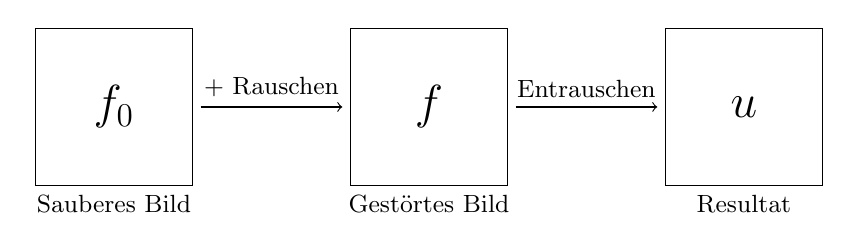
\begin{tikzpicture}
                \draw (0,0) rectangle (2,2);
                \draw (1,0) node[below] {\small Sauberes Bild};
                \draw (1,1) node[] {\LARGE $f_0$};
                \draw[->] (2.1,1) -- node[above] {\small $+$ Rauschen} (3.9,1);
                \draw (4,0) rectangle (6,2);
                \draw (5,0) node[below] {\small Gestörtes Bild};
                \draw (5,1) node[] {\LARGE $f$};
                \draw[->] (6.1,1) -- node[above] {\small Entrauschen} (7.9,1);
                \draw (8,0) rectangle (10,2);
                \draw (9,0) node[below] {\small Resultat};
                \draw (9,1) node[] {\LARGE $u$};
            \end{tikzpicture}
        \end{center}

        Wie gut das entrauschte Bild $u$ das saubere Bild $f_0$ beschreibt wird durch Normen gemessen.
	    \begin{align*}
        &\norm{f-f_0}, \text{Rauschen}\\
        &\norm{u-f_0}, \text{\textbf{Absoluter Fehler}\index{Absoluter Fehler}}\\
        &\frac{\norm{u-f_0}}{\norm{f-f_0}}, \text{\textbf{Relativer Fehler}\index{Relativer Fehler} im Vergleich zum Rauschen}\\
        &\frac{\norm{u-f_0}}{\norm{f_0}}, \text{Relativer Fehler im Vergleich zum Signal}
        \end{align*}

        Typischerweise ist die gewählte Norm:
        \[\norm{f} = \norm{f}_2 = \sqrt{\int_{\Omega} \abs{f(x)}^2 \d x}\]
        oder im diskreten:
        \[\norm{f}_2=\sqrt{\sum_{x \in \Omega} \abs{f(x)}^2}\]

        Eng verwandt ist die \textbf{Signal to noise ratio}\index{Signal to noise ratio} (SNR):
        \[\log\bigl(\underbrace{\frac{\norm{f_0}_2}{\norm{u-f_0}_2}}_{\in \ [1,\infty)}\bigr) \in [0,+\infty), \text{ wobei $0$ schlecht und $+\infty$ gut ist.}\]
    \subsection{Glättungsfilter}
        Grundidee: (zur Vereinfachung in 1D)
        \begin{center}
            \begin{tikzpicture}
                \draw (0,0) node[left] {$f_0$:};
                \draw[thick] plot [smooth, tension = 0.7] coordinates {(0,0) (1.75,1.5) (3.5,0.5) (6,2) (9,0) (11,0.5)};
                \draw[->,thick] (-0.3,-0.5) -- node[left] {Rauschen} (-0.3,-2);
                \draw (0,-2.5) node[left] {$f$:};
                \draw[thick, name path = P2,shift = {(0,-2.5)}] plot [smooth, tension = 0.7] coordinates {(0,0) (1.75,1.5) (3.5,0.5) (6,2) (9,0) (11,0.5)};
                \draw[name path = P1, draw = none] (0,-1.1) -- (3,-1.1);
                \draw[name intersections={of = P1 and P2},red,thick]
                (intersection-1) edge[bend right] ++(0.3,0.5) ++(0.3,0.5) edge[bend right] (intersection-2);
                \draw[name path = P3,draw = none] (3,-2.3) -- (5,-1.2);
                \draw[name intersections={of = P3 and P2},red,thick]
                (intersection-1) edge[bend left] ++(0.3,-0.3) ++(0.3,-0.3) edge[bend left] (intersection-2);
                \draw[] (2,-0.9) -- ++(0.5,-0.1) node[right] {\small Störungen} (3.5,-2.1) -- ++(-0.5,0.9);
                \draw (0,-5) node[left] {$f$:};
                \draw[thick, name path = P4,shift = {(0,-5)}] plot [smooth, tension = 0.7] coordinates {(0,0) (1.75,1.5) (3.5,0.5) (6,2) (9,0) (11,0.5)};
                \draw[name path = P5, shift = {(0,-2.5)}, draw = none] (0,-1.1) -- (3,-1.1);
                \draw[name intersections={of = P4 and P5},red,thick]
                (intersection-1) edge[bend right] node[black,pos=0] {\small \textbullet} ++(0.3,0.5) ++(0.3,0.5) edge[bend right] node[black,pos=1] {\small \textbullet}  node[black,pos=0] {\small \textbullet} (intersection-2);
                \draw[name path = P6, shift = {(0,-2.5)}, draw = none] (3,-2.3) -- (5,-1.2);
                \draw[name intersections={of = P4 and P6},red,thick]
                (intersection-1) edge[bend left] node[black,pos=0] {\small \textbullet} ++(0.3,-0.3) ++(0.3,-0.3) edge[bend left] node[black,pos=1] {\small \textbullet}  node[black,pos=0] {\small \textbullet} (intersection-2);
                \draw[decorate,decoration={brace,amplitude=2pt,mirror}] (1.4,-3.7) -- (2.2,-3.7);
                \draw[thick] (1.8,-3.8) -- (1.8,-4.3) node[below] {\small \framebox{Mittelwert}};
                \draw[->,thick,double] (1.6,-5) -- (0.4,-5);
                \draw[->,thick,double] (2,-5) -- (3.2,-5);
                \draw[->,thick] (1.8,-5.1) -- (1.8,-5.7);
                \draw (0,-7.5) node[left] {$u$:};
                \draw[->,thick] (-0.3,-5.5) -- node[left] {Entrauschen} (-0.3,-7);
                \draw[thick, name path = P7,shift = {(0,-7.5)}] plot [smooth, tension = 0.7] coordinates {(0,0) (1.75,1.5) (3.5,0.5) (6,2) (9,0) (11,0.5)};
                \draw[name path = P8, shift = {(0,-5)}, draw = none] (0,-1.2) -- (3,-1.2);
                \draw[name intersections={of = P7 and P8},red,thick]
                plot [smooth,tension=0.7] coordinates {(intersection-1) ($(intersection-1) + (0.5,0.35)$) (intersection-2)};
                \draw[name path = P9, shift = {(0,-5)}, draw = none] (3,-2.25) -- (5,-1.15);
                \draw[name intersections={of = P7 and P9},red,thick]
                plot [smooth,tension=0.7] coordinates {(intersection-1) ($(intersection-1) + (0.45,0.05)$) (intersection-2)};
            \end{tikzpicture}
        \end{center}

        \begin{equation} \label{eq:5.1}
            u(k) \coloneqq \alpha \cdot f(k-1) + \beta \cdot f(k) + \gamma \cdot f(k+1)
        \end{equation}
        wobei:
        \begin{equation} \label{eq:5.2}
            \alpha + \beta + \gamma = 1
        \end{equation}

        Schematisch bedeutet \eqref{eq:5.1}:

        \begin{center}
            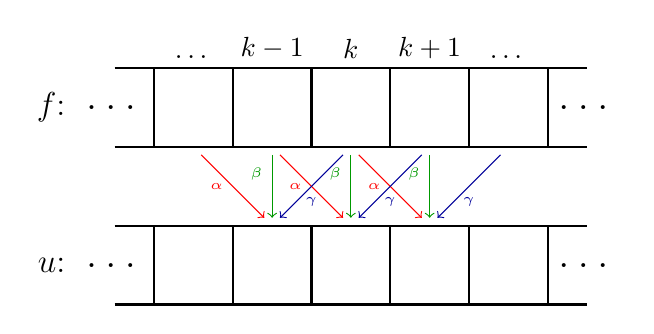
\begin{tikzpicture}
                \draw (0,-0.5) node[left] {\large $f$:};
                \draw[thick] (0.5,0) grid (6.5,-1);
                \draw (0.5,-0.5) node {\LARGE \dots};
                \draw (6.5,-0.5) node {\LARGE \dots};
                \draw (1.5,0) node[above] {\dots};
                \draw (2.5,0) node[above] {$k-1$};
                \draw (3.5,0) node[above] {$k$};
                \draw (4.5,0) node[above] {$k+1$};
                \draw (5.5,0) node[above] {\dots};
                \draw (0.5,-2.5) node {\LARGE \dots};
                \draw (6.5,-2.5) node {\LARGE \dots};

                \draw[->,red] (1.6,-1.1) -- node[left] {\tiny $\alpha$} (2.4,-1.9);
                \draw[->,red] (2.6,-1.1) -- node[left] {\tiny $\alpha$} (3.4,-1.9);
                \draw[->,red] (3.6,-1.1) -- node[left] {\tiny $\alpha$} (4.4,-1.9);
                \draw[->,black!40!green] (2.5,-1.1) -- node[left, pos = 0.3] {\tiny $\beta$} (2.5,-1.9);
                \draw[->,black!40!green] (3.5,-1.1) -- node[left, pos = 0.3] {\tiny $\beta$} (3.5,-1.9);
                \draw[->,black!40!green] (4.5,-1.1) -- node[left, pos = 0.3] {\tiny $\beta$} (4.5,-1.9);
                \draw[->,black!40!blue] (3.4,-1.1) -- node[right, pos = 0.75] {\tiny $\gamma$} (2.6,-1.9);
                \draw[->,black!40!blue] (4.4,-1.1) -- node[right, pos = 0.75] {\tiny $\gamma$} (3.6,-1.9);
                \draw[->,black!40!blue] (5.4,-1.1) -- node[right, pos = 0.75] {\tiny $\gamma$} (4.6,-1.9);

                \draw (0,-2.5) node[left] {\large $u$:};
                \draw[thick] (0.5,-2) grid (6.5,-3);
            \end{tikzpicture}
        \end{center}

        \begin{center}
            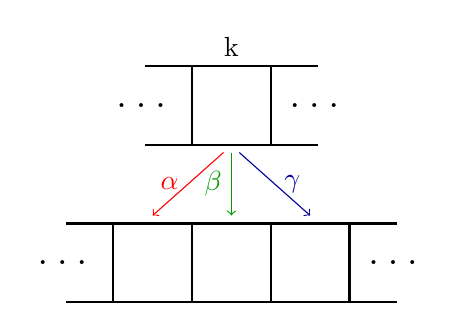
\begin{tikzpicture}
                \draw (-0.6,-0.5) node {\LARGE \dots};
                \draw (1.6,-0.5) node {\LARGE  \dots};
                \draw (-1.6,-2.5) node {\LARGE \dots};
                \draw (2.6,-2.5) node {\LARGE  \dots};
                \draw (0.5,0) node[above] {k};
                \draw[thick] (-0.6,0) grid (1.6,-1);
                \draw[->,red] (0.4,-1.1) -- node[left] {$\alpha$} (-0.5,-1.9);
                \draw[->,black!40!green] (0.5,-1.1) -- node[left] {$\beta$} (0.5,-1.9);
                \draw[->,black!40!blue] (0.6,-1.1) -- node[right] {$\gamma$} (1.5,-1.9);
                \draw[thick] (-1.6,-2) grid (2.6,-3);
            \end{tikzpicture}
        \end{center}

        Durch \eqref{eq:5.1} ist eine Abbildung $f \mapsto u$ gegeben, wir schreiben kurz:
        \[u = m \boxast f, \ \text{dieses wird \textbf{Korrelation}\index{Korrelation} genannt.}\]
        mit:
        \begin{equation}\label{eq:5.3}
            \framebox{$\displaystyle (m \boxast f)(k) = \sum_{i \in \supp(m)} m(i) f(k+i)$}
        \end{equation}
        und:
        \begin{center}
            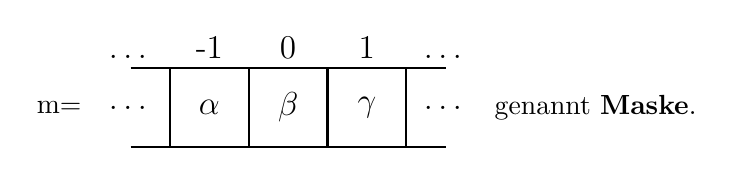
\begin{tikzpicture}
                \draw (0,0.5) node[left] {m=};
                \draw[thick] (0.5,0) grid (4.5,1);
                \draw (0.5,0.5) node {\large \dots};
                \draw (1.5,0.5) node {\large $\alpha$};
                \draw (2.5,0.5) node {\large $\beta$};
                \draw (3.5,0.5) node {\large $\gamma$};
                \draw (4.5,0.5) node {\large \dots};
                \draw (0.5,1) node[above] {\large \dots};
                \draw (1.5,1) node[above] {\large -1};
                \draw (2.5,1) node[above] {\large 0};
                \draw (3.5,1) node[above] {\large 1};
                \draw (4.5,1) node[above] {\large \dots};
                \draw (5,0.5) node[right] {genannt \textbf{Maske}\index{Maske}.};
            \end{tikzpicture}
        \end{center}

        Setzt man nun $j \coloneqq  k + i$ in \eqref{eq:5.1}, so ist $i=j-k$, d.h.
        \begin{equation}\label{eq:5.4}
            \framebox{$\displaystyle (m \boxast f)(k) = \sum_{i \in \supp(m)} m(j-k) f(j)$}
        \end{equation}

        Um die Abbildung auf den Rand anzuwenden, wird das Bild gespiegelt, in 1D:
        \begin{center}
            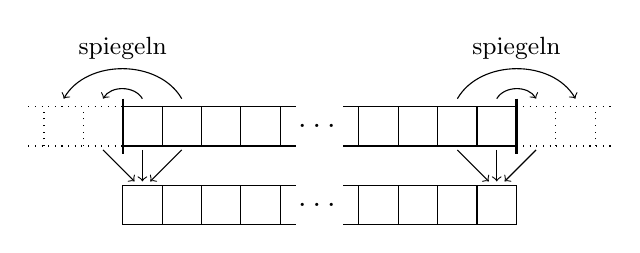
\begin{tikzpicture}
                \draw[step = 0.5] (0,0) grid (2.2,-0.5);
                \draw (2.5,-0.25) node {\large \dots};
                \draw[step = 0.5] (2.8,0) grid (5,-0.5);
                \draw[thick] (0,0.1) -- (0,-0.6);
                \draw[thick] (5,0.1) -- (5,-0.6);
                \draw[step = 0.5, dotted] (0,0) grid (-1.2,-0.5);
                \draw[step = 0.5, dotted] (5,0) grid (6.2,-0.5);
                \draw[] (0.25,0.1) edge[bend right = 60, ->] (-0.25,0.1);
                \draw[] (0.75,0.1) edge[bend right = 60, ->] node[above] {\small spiegeln} (-0.75,0.1);
                \draw[] (4.75,0.1) edge[bend left = 60, ->] (5.25,0.1);
                \draw[] (4.25,0.1) edge[bend left = 60, ->] node[above] {\small spiegeln} (5.75,0.1);
                \draw[step = 0.5] (0,-1) grid (2.2,-1.5);
                \draw (2.5,-1.25) node {\large \dots};
                \draw[step = 0.5] (2.8,-1) grid (5,-1.5);
                \draw[->] (0.25,-0.55) -- (0.25,-0.95);
                \draw[->] (-0.25,-0.55) -- (0.15,-0.95);
                \draw[->] (0.75,-0.55) -- (0.35,-0.95);
                \draw[->] (4.75,-0.55) -- (4.75,-0.95);
                \draw[->] (4.25,-0.55) -- (4.65,-0.95);
                \draw[->] (5.25,-0.55) -- (4.85,-0.95);
            \end{tikzpicture}
        \end{center}

        in 2D:
        \begin{center}
            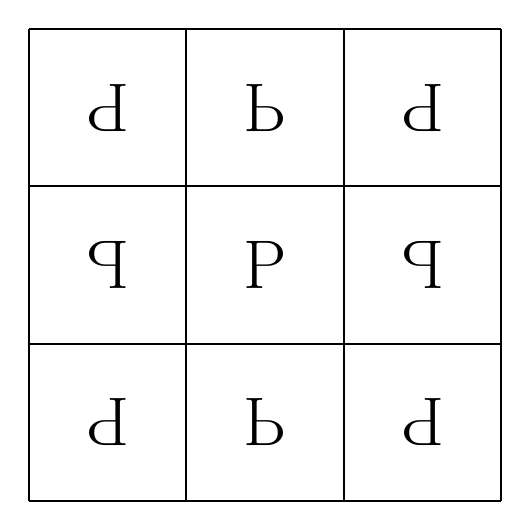
\begin{tikzpicture}
                \draw[step =2, thick] (0,0) grid (6,6);
                \draw (3,3) node {\Huge P};
                \draw (1,1) node[rotate = 180] {\Huge P};
                \draw (5,1) node[rotate = 180] {\Huge P};
                \draw (1,5) node[rotate = 180] {\Huge P};
                \draw (5,5) node[rotate = 180] {\Huge P};
                \draw (3,5) node[yscale=-1,xscale=1] {\Huge P};
                \draw (5,3) node[rotate = 180,yscale=-1,xscale=1] {\Huge P};
                \draw (1,3) node[rotate = 180,yscale=-1,xscale=1] {\Huge P};
                \draw (3,1) node[yscale=-1,xscale=1] {\Huge P};
            \end{tikzpicture}
        \end{center}

        Formel \eqref{eq:5.4} erinnert an die Formel der \textbf{Faltung}\index{Faltung}:
        \begin{equation}\label{eq:5.5}
            \framebox{$\displaystyle (g * f)(k) = \sum_{j \in \Z} g(\underbrace{k-j}_{\text{Anders als \eqref{eq:5.4}}}) \cdot f(j)$}
        \end{equation}

        Setzt man also $g(i)  \coloneqq  m(-i) =: \tilde m(i)$, was einer Spieglung der Maske entspricht, dann ist
        \[m \boxast f = g * f = \tilde m * f.\]

        Eigenschaften der Faltung:
        \begin{enumerate}[label=\framebox{\arabic *}]
            \item $(f * g) * h = f * (g* h)$, Assoziativität
            \item $f*g=g*f$, Kommutativität
            \item $\tilde f * \tilde g = \widetilde{f * g}$, Kompatibilität mit Spiegelung
        \end{enumerate}
        Eigenschaften der Korrelation:
        \begin{enumerate}[label=\framebox{\arabic *'}]
            \item $f \boxast (g \boxast h) = \tilde f * ( \tilde g* h) \overset{\framebox{\small 1}}{=} ( \tilde f * \tilde g) * h \overset{\framebox{\small 3}}{=} (\widetilde{f * g}) * h = (f * g) \boxast h \neq (f \boxast g) \boxast h$, nicht assoziativ!
            \item $f \boxast g = \tilde f * g \overset{\framebox{\small 2}}{=} g * \tilde f = \tilde{\tilde g} * \tilde f \overset{\framebox{\small 3}}{=} \widetilde{(\tilde g * f)} = \widetilde{g \boxast f} \neq g \boxast f$, nicht kommutativ!
            \item $\tilde f \boxast \tilde g = \tilde{\tilde f} * \tilde g \overset{\framebox{\small 3}}{=} \widetilde{(\tilde f * g)} = \widetilde{f \boxast g}$, Kompatibilität mit Spiegelung
        \end{enumerate}

	$\boxast$ und $*$ definiert man auf: $\ell^1(\Z^d) \coloneqq \{f=(f_i)_{i \in \Z^d} : \underbrace{\sum_{i \in \Z^d}\abs{f_i}}_{ \coloneqq \norm{f}_1} < \infty\}$

	Man kann zeigen (Übung): $f,g \in \ell^1 \Rightarrow f * g \in \ell^1$ und $\norm{f * g}_1 \leq \norm{f}_1 \C \norm{g}_1$.
    Wobei oft die Gleichheit gilt.

    Alles gilt auch in der kontinuierlichen Version:
    \[\Ell^1(\R^d)  \coloneqq  \{f:\R^d \to \R : \underbrace{\int_{\R^d}\abs{f} \d x}_{ \coloneqq \norm{f}_1} < \infty\}\]
    \[f,g \in \Ell^1(\R^d): (g*f)(x)=\int_{\R^d}g(x-y)f(y) \d y, \ y,x \in \R^d\]

    Beispiel für den kontinuierlichen Fall:
    \begin{center}
        \begin{tikzpicture}
            \draw[dotted] (0,1) node[left] {$\frac{1}{2a}$} -- (8,1);
            \draw (0,0) node[left] {$g:$} -- (2.5,0) -- (2.5,1) -- (5.5,1) -- (5.5,0) -- (8,0);
            \draw (2.5,0) node[below] {\small $-a$};
            \draw[dotted] (4,0) node[below] {\small $0$} -- (4,1.5);
            \draw (5.5,0) node[below] {\small $-a$};
        \end{tikzpicture}
    \end{center}
    Hierbei gilt $\displaystyle \int_{\R} g(x) \d x = 1$

    \begin{center}
        \begin{tikzpicture}
            \draw[thick, name path = P2] node [left] {$f:$}plot [smooth, tension = 0.45] coordinates {(0,0) (1.2,1.5) (2.1,0.3) (3,2) (4.3,1) (5.3,1.6) (6.6,0.5) (7.5,1) (8,0)};
        \end{tikzpicture}
    \end{center}

    $g \boxast f = $ \textbf{gleitendes Mittel}\index{gleitendes Mittel}.\\

        \begin{tikzpicture}
            \draw[dotted] (0,1) node[left] {$\frac{1}{2a}$} -- (8,1);
            \draw (0,0) node[left] {$g \boxast g = \tilde g * g = g * g=$} -- (1,0) -- (4,1) -- (7,0) -- (8,0);
            \draw (1,0) node[below] {\small $-2a$};
            \draw[dotted] (4,0) node[below] {\small $0$} -- (4,1.5);
            \draw (7,0) node[below] {\small $-2a$};
        \end{tikzpicture}

    Weitere Eigenschaften der Faltung:\\
    Für alle $f,g \in \Ell^1$ or $\ell ^1$
    \begin{equation*}
        \left.\begin{aligned}
            (g_1 + g_2) * f = (g_1 * f) + (g_2 * g)\\
            (\alpha g) * f = \alpha (g * f)
        \end{aligned}\right\}=\text{Linearität}
    \end{equation*}
    Somit ist:
    \[g \mapsto f * g\]
    ein linearer Operator.

    Formt $\ell^1$ bzw. $\Ell^1$ eine Algebra mit neutralem Element $\delta$?

    $\ell^1$?:
    \begin{center}
        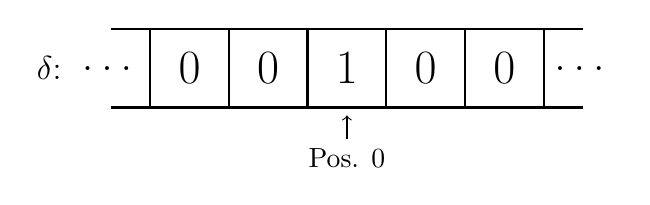
\begin{tikzpicture}
            \draw (0,-0.5) node[left] {\large $\delta$:};
            \draw[thick] (0.5,0) grid (6.5,-1);
            \draw (0.5,-0.5) node {\LARGE \dots};
            \draw (6.5,-0.5) node {\LARGE \dots};
            \draw (1.5,-0.5) node {\LARGE 0};
            \draw (2.5,-0.5) node {\LARGE 0};
            \draw (3.5,-0.5) node {\LARGE 1};
            \draw (4.5,-0.5) node {\LARGE 0};
            \draw (5.5,-0.5) node {\LARGE 0};
            \draw[->] (3.5,-1.4) node[below] {Pos. $0$} -- (3.5,-1.1);
        \end{tikzpicture}
    \end{center}
    Ja!

    $\Ell^1$?:
    Für ein solches Element muss gelten:\\
    $\forall f \in \Ell^1 : d * f = f$\\
    $\forall x \in \R :\displaystyle \int_{\R^d} \underbrace{\delta(x-y)}_{=0 \forall x \neq y} f(y) \d y = f(x)$

    Diese Funktion wird \textbf{Dirac-Impuls}\index{Dirac-Impuls} genannt ist aber kein Element von $\Ell^1$.

    \pa{Nun zu Masken in 2D:}

    \begin{equation*}
        u = m \boxast f \text{ mit } m= \raisebox{-0.665cm}{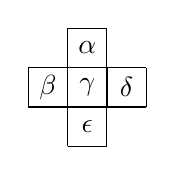
\begin{tikzpicture}
            \draw[step = 0.5] (0,0) grid (0.5,1.5);
            \draw[step = 0.5] (-0.5,1) grid (1,0.5);
            \draw (0.25,1.25) node {$\alpha$};
            \draw (0.25,0.75) node {$\gamma$};
            \draw (0.25,0.25) node {$\epsilon$};
            \draw (-0.25,0.75) node {$\beta$};
            \draw (0.75,0.75) node {$\delta$};
        \end{tikzpicture}}
    \end{equation*}
    wobei $\alpha + \beta +\gamma +\delta + \epsilon = 1$\\
    Kurzschreibweise: $u_{ij} \coloneqq u(x)$ wobei $x = \begin{pmatrix}i\\j\end{pmatrix} \in \Z^2$, analog für $f_{ij}$.
    \[\Rightarrow u_{ij} = \alpha f_{i-1,j} + \beta f_{i,j-i} + \gamma f_{ij} + \delta f_{i,j+1} + \epsilon f_{i+1,j}\]

    \begin{equation*}
        u = m \boxast f = \tilde m * f \text{ mit } \tilde m = \raisebox{-0.665cm}{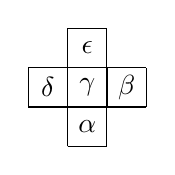
\begin{tikzpicture}
            \draw[step = 0.5] (0,0) grid (0.5,1.5);
            \draw[step = 0.5] (-0.5,1) grid (1,0.5);
            \draw (0.25,1.25) node {$\epsilon$};
            \draw (0.25,0.75) node {$\gamma$};
            \draw (0.25,0.25) node {$\alpha$};
            \draw (-0.25,0.75) node {$\delta$};
            \draw (0.75,0.75) node {$\beta$};
        \end{tikzpicture}}
    \end{equation*}

    \pa{Symmetrischer Fall:}

    \begin{equation*}
    \tilde m = \raisebox{-0.665cm}{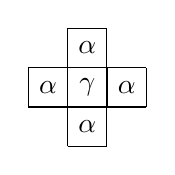
\begin{tikzpicture}
            \draw[step = 0.5] (0,0) grid (0.5,1.5);
            \draw[step = 0.5] (-0.5,1) grid (1,0.5);
            \draw (0.25,1.25) node {$\alpha$};
            \draw (0.25,0.75) node {$\gamma$};
            \draw (0.25,0.25) node {$\alpha$};
            \draw (-0.25,0.75) node {$\alpha$};
            \draw (0.75,0.75) node {$\alpha$};
        \end{tikzpicture}} \text{ mit } \gamma = 1 - 4 \alpha
    \end{equation*}

    \begin{equation}
        u_{ij} = (1 - 4 \alpha)f_{ij} + \alpha(f_{i-1,j} + f_{i,j-1} + f_{i,j+1} + f_{i+1,j})
    \end{equation}

    \begin{equation*}
            \text{Erinnerung: } \raisebox{-1.2cm}{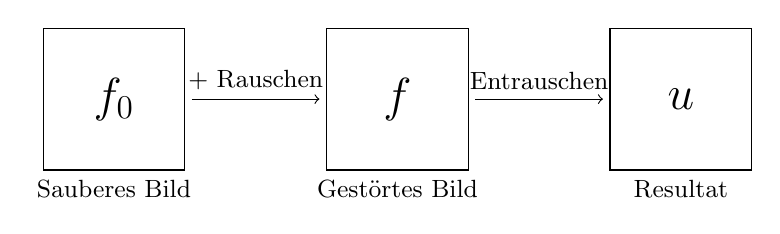
\begin{tikzpicture}[scale=0.9]
                \draw (0,0) rectangle (2,2);
                \draw (1,0) node[below] {\small Sauberes Bild};
                \draw (1,1) node[] {\LARGE $f_0$};
                \draw[->] (2.1,1) -- node[above] {\small $+$ Rauschen} (3.9,1);
                \draw (4,0) rectangle (6,2);
                \draw (5,0) node[below] {\small Gestörtes Bild};
                \draw (5,1) node[] {\LARGE $f$};
                \draw[->] (6.1,1) -- node[above] {\small Entrauschen} (7.9,1);
                \draw (8,0) rectangle (10,2);
                \draw (9,0) node[below] {\small Resultat};
                \draw (9,1) node[] {\LARGE $u$};
            \end{tikzpicture}}
    \end{equation*}

    Wir nehmen an, dass $f_{ij} = f_{ij}^0 +\delta_{ij}$ gilt mit $\delta_{ij} \sim N(0,\sigma^2)$ iid (additives Gauß'sches Rauschen). 

    Wir wollen zeigen: $\var(u_{ij}) \leq \var(f_{ij})$

    \begin{align*}
        \var(f_{ij}) 
        &= \Ew(\underbrace{f_{ij} - \overbrace{E f_{ij}}^{f^0_{ij}}}_{r_{ij}})^2 
        = \sigma^2 \\
        %
        \var(u_{ij}) 
        &= \Ew(u_{ij} - \Ew u_{ij})^2  \\
        &= \Ew\Big( (\Big( (1 - 4\alpha) (f_{ij} - \Ew f_{ij} ) \Big)  + \alpha \Big( ( f_{i - 1, j} - \Ew f_{i- 1, j}) + \cdots + (f_{i + 1, j} - \Ew f_{i + 1, j}) \Big) \Big)^2 \\
        &= \Ew \Big( (1 - 4\alpha) \delta_{ij} + \alpha ( \delta_{i - 1, j} + \delta_{i, j - 1} + \delta_{i, j+ 1} + \delta_{i + 1, j}) \Big)^2 \\
        &= (1 - 4\alpha)^2 \sigma^2 + 4 \alpha^2 \sigma^2 \\
        &= (1 - 8\alpha + 20\alpha^2) \sigma^2.
%        = \Ew((1 - 4 \alpha) (\underbrace{f_{ij} - f^0_{ij}}_{r_{ij}}) + \alpha(\underbrace{(f_{i-1,j} - f^0_{i-1,j})}_{r_{i-1,j}} + \cdots + \underbrace{(f_{i+1,j} - f^0_{i+1,j})}_{r_{i+1,j}}))^2\\
%        &= \Ew((1 - 4 \alpha)^2 r_{ij}^2 + \alpha^2(r_{i-1,j}^2 + r_{i,j-1}^2 +r_{i,j+1}^2 + r_{i+1,j}^2) + 2 (1 - 4 \alpha) \alpha r_{ij} r_{i-1,j}\dots)\\%TODO fix this mess
%        &= (1 - 4 \alpha)^2 \underbrace{\Ew r_{i,j}^2}_{\sigma^2} + \alpha^2(\Ew r_{i-1,j}^2 + \dots + \Ew r_{i+1,j}^2) + 2 (1 - 4 \alpha) \alpha \underbrace{\Ew(r_{ij}r_{i-1,j})}_{\underbrace{\Ew r_{ij} \Ew r_{i-1,j}}_{0}} + \underbrace{\dots}_{0})\\
%        &=(1 - 4 \alpha)^2 \sigma^2 + \alpha^2 4 \sigma^2 = (1 - 8 \alpha + 16 \alpha ^2 + 4 \alpha^2) \sigma^2
    \end{align*}

    Da $0 \leq \alpha$ und $ 0 \leq 1 - 4 \alpha \Rightarrow 0 \leq \alpha \leq \frac{1}{4}$:

    \begin{equation*}
        (1 - 8 \alpha + 16 \alpha ^2 + 4 \alpha^2) \sigma^2 = \underbrace{1 + \underbrace{20 \alpha}_{\geq 0} (\underbrace{\alpha - \frac{2}{5}}_{< 0})}_{\leq 1}
    \end{equation*}

    $\Rightarrow \var(u_{ij}) \leq \var(f_{ij})$ für $\alpha \in [0,\frac{1}{4}]$\\

    Dabei gilt: $\var(u_{ij}) \overset{\alpha}{\to} \text{min} \iff 1 - 8 \alpha + 20 \alpha^2 \overset{\alpha}{\to} \text{min} \iff -8 + 40 \alpha = 0 \iff \alpha = \frac{1}{5}$
    \begin{equation*}
        \Rightarrow \text{bester Filter} : \ \raisebox{-0.9cm}{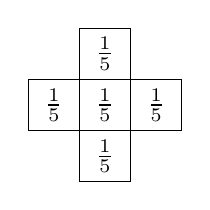
\begin{tikzpicture}[scale = 1.3]
                \draw[step = 0.5] (0,0) grid (0.5,1.5);
                \draw[step = 0.5] (-0.5,1) grid (1,0.5);
                \draw (0.25,1.25) node {$\frac{1}{5}$};
                \draw (0.25,0.75) node {$\frac{1}{5}$};
                \draw (0.25,0.25) node {$\frac{1}{5}$};
                \draw (-0.25,0.75) node {$\frac{1}{5}$};
                \draw (0.75,0.75) node {$\frac{1}{5}$};
            \end{tikzpicture}}
        \end{equation*}

    \subsection{Frequenzraum-filter}
        Ansatz: Rauschen = hochfrequente Anteile des Signals.\\
        Diese können mittels der \textbf{Fouriertransformation}\index{Fouriertransformation} $\mathcal F$ gezielt entfernt werden.
        \begin{equation*}
            \begin{tikzpicture}[scale = 0.9]
                \draw (0,0) rectangle (2,2);
                \draw (1,0) node[below] {\small Sauberes Bild};
                \draw (1,1) node[] {\LARGE $f_0$};
                \draw[->] (2.1,1) -- node[above] {$+r$} (2.9,1);
                \draw (3,0) rectangle (5,2);
                \draw (4,0) node[below] {\small Gestörtes Bild};
                \draw (4,1) node[] {\LARGE $f$};
                \draw[->] (5.1,1) -- node[above] {$\mathcal F$} (5.9,1);
                \draw (6,-0.5) rectangle (9,2.5);
                \draw (6,1) -- (9,1);
                \draw[thick, name path = P2]plot [smooth, tension = 0.8] coordinates {(6,1) (6.1,1.3) (6.4,1.1) (6.6,1.6) (7,1.1) (7.3,2.0) (7.5,1.1) (7.7,1.2) (7.8,1.9) (8.1,1.5) (8.5,1.9) (9,1)};
                \draw[->] (9.1,1) -- node[above] {\small Abschneiden} (10.9,1);
                \draw[->] (14.1,1) -- node[above] {$\mathcal F^{-1}$} (14.9,1);
                \draw[decorate,decoration={brace,amplitude=2pt,mirror}] (6,0.6) -- node[below] {\scriptsize \begin{tabular}{c} niedrige \\ Frequenzen \end{tabular}} (7.5,0.6);
                \draw[decorate,decoration={brace,amplitude=2pt,mirror}] (7.5,0.6) -- node[below] {\scriptsize \begin{tabular}{c} hohe \\ Frequenzen \end{tabular}} (9,0.6);
                \draw[thick, name path = P2,shift = {(5,0)}]plot [smooth, tension = 0.8] coordinates {(6,1) (6.1,1.3) (6.4,1.1) (6.6,1.6) (7,1.1) (7.3,2.0) (7.5,1.1) (7.7,1.2) (7.8,1.9) (8.1,1.5) (8.5,1.9) (9,1)};
                \draw[color = white,fill] (12.7,1) rectangle (14,2.5);
                \draw (11,1) -- (14,1);
                \draw (11,-0.5) rectangle (14,2.5);
                \draw (15,0) rectangle (17,2);
                \draw[thick] (7.7,0.8) -- (7.7,2.3);
                \draw[thick] (12.7,0.8) -- (12.7,2.3);
                \draw (16,1) node[] {\LARGE $u$};
                \draw[decorate,decoration={brace,amplitude=2pt,mirror}] (5.5,-1) -- node[below] {im Frequenzbereich} (14.5,-1);
                \draw[decorate,decoration={brace,amplitude=2pt,mirror}] (3,-1.5) -- node[below] {\textbf{Frequenzraumfilter}\index{Frequenzraumfilter} (Tiefpass)} (17,-1.5);
            \end{tikzpicture}
    \end{equation*}

    Ein wichtiges Instrument ist hierbei die Fouriertransformation:
    \[\mathcal F : f \mapsto \hat f\]
    \begin{equation}
        \boxed{\hat f(z) = \frac{1}{(2 \pi)^\frac{d}{2}} \int_{\R^d} f(x) \e^{-\ii \skprod{z}{x}} \d x}
    \end{equation}

    Wobei  $z \in \R^d, f \in \Ell^1(\R^d)$.

    Falls auch $\hat f \in \Ell^1(\R^d)$ ist ,dann lässt sich $f$ wie folgt mittels der inversen Fouriertransformation aus $\hat f$ rekonstruieren:
    \[\mathcal F^{-1} : \hat f \mapsto f\]
    \begin{equation}
        \boxed{f(z) = \frac{1}{(2 \pi)^\frac{d}{2}} \int_{\R^d} \hat f(x) \e^{\ii \skprod{z}{x}} \d x}
    \end{equation}
    Wobei $x \in \R^d$.\\

    Man hat also $\mathcal F^{-1} \mathcal F f$, d.h.
    \[f(x) = \frac{1}{(2 \pi)^\frac{d}{2}} \int_{\R^d} \left(\frac{1}{(2 \pi)^\frac{d}{2}} \int_{\R^d} f(y) \e^{-\ii \skprod{z}{y}} \d y\right) \e^{\ii \skprod{z}{x}} \d z\]

    Sei nun $e_z(x)  \coloneqq  \e^{\ii \skprod{z}{x}}, \ x \in \R^d$ mit Parameter
$z = \srmatrix{z_1 \\ \vdots \\ z_d}$.\\
    Also $e_z(x) = \e^{\ii\skprod{\srmatrix{z_1\\z_2}}{\srmatrix{x_1\\x_2}}} 
    = \e^{\ii (z_1 x_1 +z_2 x_2)}$\\
    Beispiele in $2D$:\\
    (Hier stellen die Linien, Punkte mit konstantem wert dar)

    \begin{minipage}[t]{0.49\linewidth}
        \begin{center}
            $z = \srmatrix{1 \\ 0}, \  \e_z(x)=\e^{\ii x_1}$:\\
            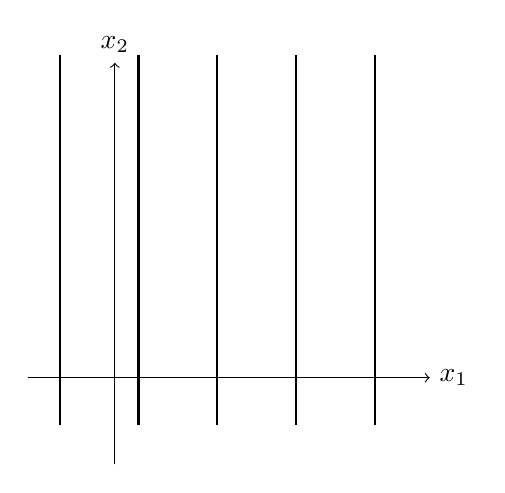
\begin{tikzpicture}
                \draw[->] (-1.1,0) -- (4,0) node[right] {$x_1$};
                \draw[->] (0,-1.1) -- (0,4) node[above] {$x_2$};
                \foreach \i in {-0.7, 0.3, 1.3, 2.3, 3.3}{
                    \draw[thick] (\i,-0.6) -- (\i,4.1);
                }
            \end{tikzpicture}

            $z = \srmatrix{0 \\ 1}, \  e_z(x)=\e^{\ii x_2}$:\\
            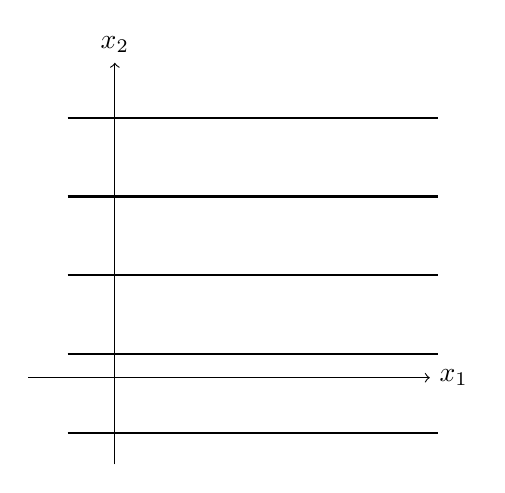
\begin{tikzpicture}
                \draw[->] (-1.1,0) -- (4,0) node[right] {$x_1$};
                \draw[->] (0,-1.1) -- (0,4) node[above] {$x_2$};
                \foreach \i in {-0.7, 0.3, 1.3, 2.3, 3.3}{
                    \draw[thick] (-0.6,\i) -- (4.1,\i);
                }
            \end{tikzpicture}

            $z = \srmatrix{1 \\ 1}, \  e_z(x)=\e^{\ii(x_1 + x_2}$:\\
            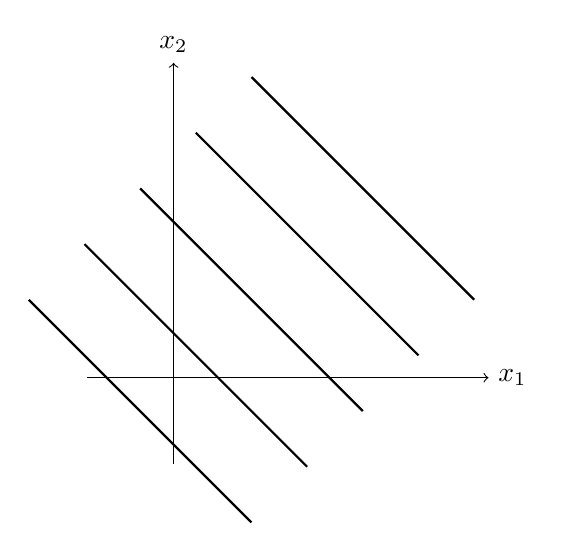
\begin{tikzpicture}
                \draw[->] (-1.1,0) -- (4,0) node[right] {$x_1$};
                \draw[->] (0,-1.1) -- (0,4) node[above] {$x_2$};
                \foreach \i in {-2.6, -1.6, -0.6, 0.4, 1.4}{
                    \draw[thick, rotate = -45,shift={(0,\i)}] (-2,2) -- (2,2);
                }
            \end{tikzpicture}
        \end{center}
    \end{minipage}
    \hfill
    \begin{minipage}[t]{0.49\linewidth}
        $z = \srmatrix{2 \\ 0}, \ \e_z(x)=\e^{\ii 2x_1}$:\\
        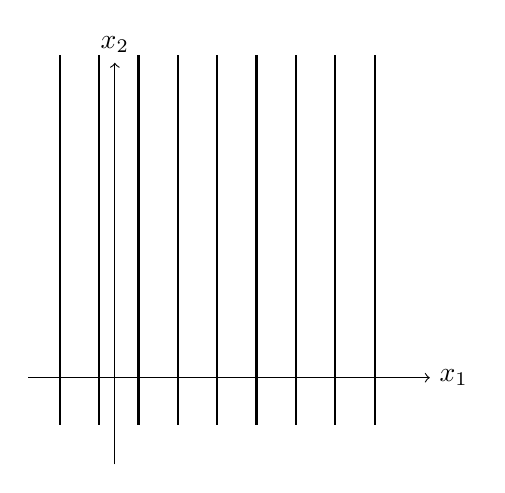
\begin{tikzpicture}
            \draw[->] (-1.1,0) -- (4,0) node[right] {$x_1$};
            \draw[->] (0,-1.1) -- (0,4) node[above] {$x_2$};
            \foreach \i in {-0.7, -0.2, 0.3, 0.8, 1.3, 1.8, 2.3, 2.8, 3.3}{
                \draw[thick] (\i,-0.6) -- (\i,4.1);
            }
        \end{tikzpicture}

        $z = \srmatrix{0 \\ 2}, \  \e_z(x)=\e^{\ii 2x_2}$:\\
        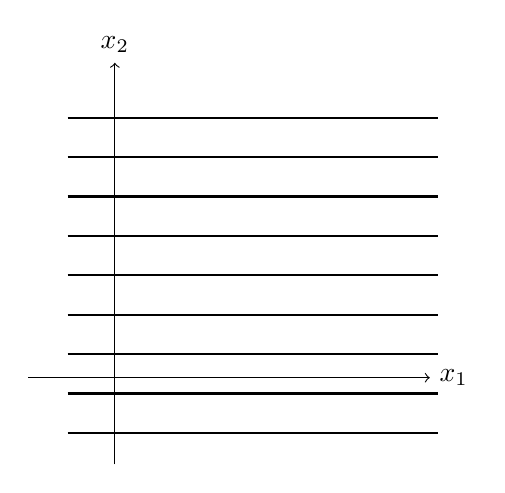
\begin{tikzpicture}
            \draw[->] (-1.1,0) -- (4,0) node[right] {$x_1$};
            \draw[->] (0,-1.1) -- (0,4) node[above] {$x_2$};
            \foreach \i in {-0.7, -0.2, 0.3, 0.8, 1.3, 1.8, 2.3, 2.8, 3.3}{
                \draw[thick] (-0.6,\i) -- (4.1,\i);
            }
        \end{tikzpicture}

        $z = \srmatrix{-2 \\ 1}, \  \e_z(x)=\e^{\ii(-2x_1 + x_2)}$:\\
        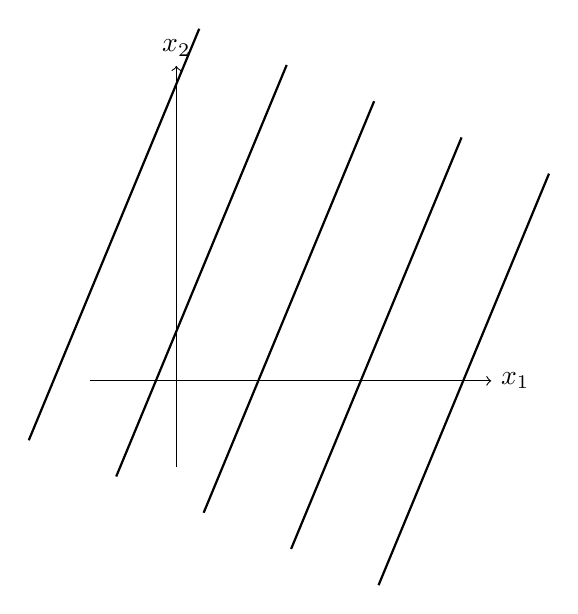
\begin{tikzpicture}
            \draw[->] (-1.1,0) -- (4,0) node[right] {$x_1$};
            \draw[->] (0,-1.1) -- (0,4) node[above] {$x_2$};
            \foreach \i in {-2.8, -1.8, -0.8, 0.2, 1.2}{
                \draw[thick, rotate = 112.5,shift={(0.85*\i,0.85*\i)}] (-1,1) -- (3,-3);
            }
        \end{tikzpicture}
    \end{minipage}

    $\displaystyle f \in \Ell^2(\R^d) = \{f:\R^d \to \R | \int_{\R^d} \abs{f}^2 \d x < \infty\}$ ist
    \begin{enumerate}[label = -]
        \item ein normierter Raum mit $+$, $\alpha \cdot$ und $\displaystyle \norm{\cdot}_2  \coloneqq  \sqrt{\int_{\R^d} \abs{f(x)}^2 \d x}$
        \item ein Skalarproduktraum mit $\displaystyle \skprod{f}{g}  \coloneqq  \int_{\R^d} f \bar g \ \d x$, wobei $\norm{f}_2^2=\skprod{f}{f}$
        \item ein vollständiger metrischer Raum, also ein \textbf{Banachraum}\index{Banachraum}
    \end{enumerate}
    Ein vollständiger normierter Banachraum mit Skalarprodukt heißt \textbf{Hilbertraum}\index{Hilbertraum}.

    $\mathcal F$ kann auch als Abbildung auf $\Ell^2(\R^d)$ betrachtet werden. Dann gilt:\\
    \[\hat f = \mathcal F f \in \Ell^2(\R^d)\]
    und
    \begin{equation}
        \| \hat f \|_2 = \norm{f}_2
    \end{equation}
    und sogar
    \begin{equation}
        \skprod{\hat f}{\hat g}_2 = \skprod{f}{g}_2
    \end{equation}
    für alle $f,g \in \Ell^2(\R^d)$.

    Weitere Eigenschaften der Fouriertransformation:
    \begin{enumerate}[label = \roman *)]
        \item $f \in \Ell^1(\R^d) \Rightarrow \hat f$ stetig und $\underset{\abs{z} \to \infty}{\lim} \hat f(z) = 0$
        \item $\mathcal F: \Ell^1(\R^d) \to \CC(\R^d)$ ist eine lineare Abbildung
        \item $\mathcal F: \Ell^1(\R^d) \to \CC(\R^d)$ ist eine beschränkte/stetige Abbildung
        \item Verschiebung $\overset{\mathcal F}{\to}$ Modulation, d.h.
        \begin{equation*}
            g(x) = f(x+a) \Rightarrow \hat g(z) = \e^{\ii \skprod{a}{z}} \hat f(z)
        \end{equation*}
        \item Modulation $\overset{\mathcal F}{\to}$ Verschiebung, d.h.
        \begin{equation*}
            g(x) = \e^{\ii \skprod{x}{a}} f(x) \Rightarrow \hat g(z)= \hat f(z-a)
        \end{equation*}
        \item Skalierung $\overset{\mathcal F}{\to}$ inverse Skalierung, d.h.
        \begin{equation*}
            g(x)=f(cx) \Rightarrow \hat g(z) = \frac{1}{\abs c} \hat f\left(\frac{z}{\abs c}\right)
        \end{equation*}
        \item Konjugation: $g(x) = \overline{f(x)} \Rightarrow \hat g(z) = \overline{\hat f (-z)}$\\
        Folglich: $f$ reelwertig $\Rightarrow \hat f(z) = \overline{\hat f(-z)}$
        \item
        \begin{align*}
            \text{Grundmode:} \ & \displaystyle \hat f(0) = \frac{1}{(2 \pi )^\frac{d}{2}} \int_{\R^d} f(x) \d x\\
            \text{Analog:} \ & \displaystyle f(0) = \frac{1}{(2 \pi )^\frac{d}{2}} \int_{\R^d} \hat f(x) \d x
        \end{align*}
        \item Differentiation $\overset{\mathcal F}{\to}$ Multiplikation mit Potenzen von z, d.h.
        \begin{equation*}
            g(x) = \frac{\partial^{\alpha_1 + \cdots + \alpha_d}}{\partial x_1^{\alpha_1} \cdots \partial x_d^{\alpha_d}} f(x) \Rightarrow \hat g(z) = i^{\alpha_1 + \cdots + \alpha_d} z_1^{\alpha_1} \cdots z_d^{\alpha_d} \hat f(z)
        \end{equation*}
        \item Umkehrung des letzten Punktes:
        \begin{equation*}
            g(x) = x_1^{\alpha_1} \cdots x_d^{\alpha_d} f(x) \Rightarrow \hat g(z) = i^{\alpha_1 + \cdots + \alpha_d}  \frac{\partial^{\alpha_1 + \cdots + \alpha_d}}{\partial x_1^{\alpha_1}} \hat f(z)
        \end{equation*}
        \item
        \begin{align*}
            \text{Faltungssatz:} \  & \mathcal F(f*g) = (2 \pi)^{\frac{d}{2}} \mathcal F(f) \cdot \mathcal F(g), \ \widehat{f*g}=(2 \pi)^{\frac{d}{2}} \hat f \cdot \hat g\\
            \text{Analog:} \ & \mathcal F (f \cdot g) = \frac{1}{(2 \pi)^{\frac{d}{2}}} \mathcal F(f) * \mathcal F(g), \ \widehat{f \cdot g} = \frac{1}{(2\pi)^{\frac{d}{2}}} \hat f * \hat g
        \end{align*}
        d.h.: Faltung $\overset{\mathcal F}{\to}$ Multiplikation und umgekehrt
    \end{enumerate}

    \Large{\textbf{Zur Erinnerung:}}
    \normalsize
    \begin{center}
        \begin{tikzpicture}[scale = 0.9]
            \draw (0,0) rectangle (3,3);
            \draw (1.5,1.5) node[] {\LARGE $f_0$};
            \draw[->] (3.1,1.5) -- node[above] {$\mathcal F$} (3.9,1.5);
            \draw (4,0) rectangle (7,3);
            \draw (5.5,1.5) node[] {\LARGE $\hat f$};
            \draw[->] (7.1,1.5) -- node[above] {\footnotesize \begin{tabular}{c}
                Hohe Frequenzen\\abschneiden
            \end{tabular}} (9.4,1.5);
            \draw (9.5,0) rectangle (12.5,3);
            \draw (11,1.5) node[] {\LARGE $\hat u$};
            \draw[->] (12.6,1.5) -- node[above] {$\mathcal F^{-1}$} (13.4,1.5);
            \draw (13.5,0) rectangle (16.5,3);
            \draw (15,1.5) node[] {\LARGE $u$};

            \draw[thin] (4,-2) -- node[below] {\small 0} (7,-2);
            \draw[thick, name path = P2,shift = {(-2,-3)}]plot [smooth, tension = 0.8]coordinates {(6,1) (6.1,1.3) (6.4,1.1) (6.6,1.6) (7,1.1) (7.3,2.0) (7.5,1.1) (7.7,1.2) (7.8,1.9) (8.1,1.5) (8.5,1.9) (9,1)};
            \draw[decorate,decoration={brace,amplitude=2pt,mirror}] (4.8,-2.5) -- node[below] {\small tiefe Frequenzen} (6.2,-2.5);

            \draw[thick, name path = P2,shift = {(3.5,-3)}]plot [smooth, tension = 0.8]coordinates {(6,1) (6.1,1.3) (6.4,1.1) (6.6,1.6) (7,1.1) (7.3,2.0) (7.5,1.1) (7.7,1.2) (7.8,1.9) (8.1,1.5) (8.5,1.9) (9,1)};
            \draw[fill, color = white] (9.5,-2) rectangle (10.3,-0.5);
            \draw[fill, color = white] (12.5,-2) rectangle (11.7,-0.5);
            \draw[] (11.7,-0.7) -- (11.7,-2.1) node[below] {\small $r$};
            \draw[] (10.3,-0.7) -- (10.3,-2.1) node[below] {\small $-r$};
            \draw[thin] (9.5,-2) -- (12.5,-2);
            \draw (11,-2.1) node[below] {\small 0};

            \draw[->] (5.5,-3) -- (5.5,-3.5) -- (11,-3.5) -- (11,-2.7);

            \draw[shift = {(0.25,-0.3)}] (6.25,-3.8) node[] {\small \textbullet} (6.5,-4) -- (7,-4) node[below] {\small $-r$} -- (7,-3.6) -- (9,-3.6) -- (9,-4) node[below] {\small $r$} -- (9.5,-4) (8,-4) node[below] {\small 0};

        \end{tikzpicture}
    \end{center}

    \begin{center}
        \begin{tikzpicture}
            \draw[dotted] (-0.3,0) rectangle (-6,-7);
            \draw (-2.5,0) node[above] {\textbf{Zeitbereich}\index{Zeitbereich}};
            \draw[dotted] (0.3,0) rectangle (6,-7);
            \draw (2.5,0) node[above] {\textbf{Frequenzbereich}\index{Frequenzbereich}};

            \draw (-3,-1) node[] {$f$};
            \draw (-2.8,-1) edge[bend right=-15,->] node[above, pos = 0.5] {$\mathcal F$} node[below, pos = 0.5] {\small $n \C \log(n)$} (2.8,-1);
            \draw (3,-1) node[] {$\hat f$};
            \draw[] (3,-1.5) edge[bend right=-15,->] node[right, pos = 0.5] {\small Mult. mit:} node[left, pos = 0.5] {\small $n$} (3,-5.5);
            \draw (4.05,-4) node[left] {\footnotesize $\hat g \coloneqq $};
            \draw (4,-4.1) -- (4.3,-4.1) -- (4.3,-3.8) -- (5,-3.8) -- (5,-4.1) -- (5.3,-4.1) (4.65,-4.1) node[] {\tiny $0$};
            \draw[dotted] (4,-3.8) -- (5.3,-3.8) node[xshift=10] {\footnotesize $\frac{1}{(2 \pi)^\frac{d}{2}}$};
            \draw (3,-6) node[] {$\hat u$} (3,-6.25) node[right] {\small \begin{tabular}{c}
                $= \hat f \cdot \hat g \cdot (2 \pi)^{\frac{d}{2}}$\\
                $= \widehat{f*g}$
            \end{tabular}};
            \draw[] (2.5,-6) edge[bend right=-15,->] node[above, pos = 0.5] {\small $n \cdot \log(n)$} node[below, pos = 0.5] {$\mathcal F^{-1}$} (-2.5,-6);
            \draw (-3,-6) node[] {$u$};
            \draw (-3,-6) node[left] {\small $f*g=$};
            \draw (-3,-1.5) edge[bend left=-15,->] node[right,pos = 0.5] {\small $n^2$} node[left, pos = 0.5] {\small Faltung, $*g$} (-3,-5.5);
            \draw [thick, name path = P2,->]plot [smooth, tension = 0.9]coordinates {(-2.5,-1.5) (1.5,-1.5) (1.5,-5) (-2.5,-5.5)};
            \draw (2,-3.5) node[left] {\small $n \cdot \log(n)$};
        \end{tikzpicture}
    \end{center}

    Wie sieht $g$ aus?
    \[g = \mathcal F^{-1} \left(\frac{1}{( 2 \pi)^{\frac{d}{2}}} \chi_{[-r,r]}\right), \quad 
        \chi_M(z) =
        \begin{cases}
             0, & z \not \in M\\
             1, & z \in M
        \end{cases}\]

    \normalsize
    \begin{align*}
        g(x) = & \frac{1}{( 2 \pi)^{\frac{d}{2}}}(\mathcal F^{-1} \chi_{[-r,r]^d})(x)\\
        = & \frac{1}{( 2 \pi)^{\frac{d}{2}}} \frac{1}{( 2 \pi)^{\frac{d}{2}}} \int_{\R^d} \chi_{[-r,r]^d}(z) \e^{\ii \skprod{z}{x}} \d z\\
        (d=1) \to = & \frac{1}{2 \pi} \int_{-\infty}^{\infty} \chi_{[-r,r]}(z) \e^{\ii zx} \d z = \frac{1}{2 \pi} \int_{r}^{-r} \e^{\ii zx} \d z\\
        = & \frac{1}{2 \pi}  \frac{\e^{\ii zx}}{\ii x} \Big|_{z=-r}^{r} = \frac{1}{2 \pi \ii x}\left( \e^{\ii rx} - \e^{-\ii rx} \right)\\
        = & \frac{1}{\pi x} \sin(rx) = \sinc\left(\frac{rx}{\pi}\right) \cdot \frac{r}{\pi}
    \end{align*}

    \[\text{Wobei:\ } \sinc(\varphi)=
    \begin{cases}
        \frac{\sin(\pi \varphi)}{\pi \varphi} &, \varphi \neq 0\\
        1 &, \varphi = 0
    \end{cases}\]

    $g$ hat auch Masse $1$, denn mit den Eigenschaften der Fouriertransformation folgt:
    \[\frac{1}{( 2 \pi)^{\frac{d}{2}}} = \hat g(0) = (\mathcal F g)(0) = \frac{1}{( 2 \pi)^{\frac{d}{2}}} \int_{R^d} g(x) \underbrace{\e^{-\overbrace{\skprod{x}{0}}^0}}_1 \d x = \frac{1}{( 2 \pi)^{\frac{d}{2}}} \int_{R^d} g(x) \d x\]
    \[\Rightarrow \int_{\R^d} g(x) \d x = 1\]

    Für $d=2$ gilt:
    \begin{align*}
        g(x) = & \frac{1}{(2 \pi)^{1}}(\mathcal F^{-1} \chi_{[-r,r]^2})(x)\\
        = & \ \cdots \ (\text{Analog zu oben})\\
        = & \frac{1}{(2 \pi)^{2}} \int_{-\infty}^\infty  \int_{-\infty}^\infty \chi_{[-r,r]^2}\left( \srmatrix{x_1\\x_2} \right) \e^{\ii (z_1 x_1 + z_2 x_2)} \d z_1 \d z_2\\
        = & \frac{1}{(2 \pi)^{2}} \int_{-r}^r \left( \int_{-r}^r \e^{\ii z_1 x_1} \e^{\ii z_2 x_2} \d z_1 \right)\d z_2\\
        = & \underbrace{ \left(\frac{1}{2 \pi} \int_{-r}^r \e^{\ii z_1 x_1} \d z_1\right) }_{\frac{1}{\pi x_1} sin(\pi x_1)} \underbrace{ \left( \frac{1}{2 \pi} \int_{-r}^r \e^{\ii z_2 x_2} \d z_2 \right)}_{\frac{1}{\pi x_2} sin(\pi x_2)}\\
    \end{align*}

    Es ist zu bemerken, dass $g$ eine Art Tensor Struktur besitzt, was in etwa bedeutet das sich die Funktion in beliebigen Dimensionen als Produkt der Funktion in einer Dimensionen darstellen lässt.

    \textbf{Gauß-Kern}\index{Gauß-Kern}:
    \begin{align*}
        G(x) =& \frac{1}{(2 \pi)^{\frac{d}{2}}} \e^{\frac{-\abs{x}^2}{2}} \Rightarrow G\left( \srmatrix{x_1\\\vdots\\x_d} \right) = \frac{1}{(2 \pi)^{\frac{d}{2}}} \e^{\frac{-x_1^2-x_2^2 - \cdots - x_d^2}{2}}\\
        =& \left( \frac{1}{(2 \pi)^\frac{1}{2}} \e^{\frac{-x_1^2}{2}}\right) \cdot \ \cdots \ \cdot \left( \frac{1}{(2 \pi)^\frac{1}{2}} \e^{\frac{-x_d^2}{2}}\right) = G(x_1) \cdot \ \cdots \ \cdot G(x_d)
    \end{align*}

    \subsection{Filterbreite und Glättung}

    \begin{center}
        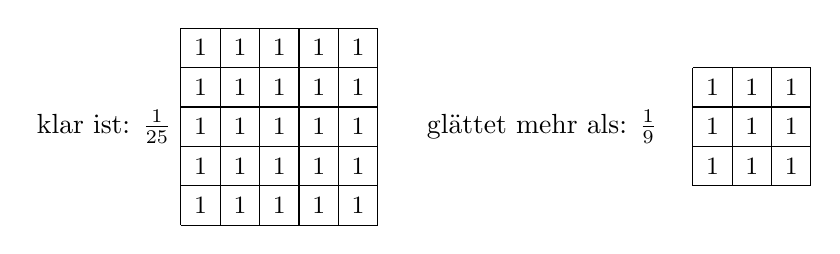
\begin{tikzpicture}
            \foreach \i in {0,...,4}
                \foreach \j in {0,...,4}
                    \draw (0.5*\i + 0.25,0.5*\j + 0.25) node[] {\small 1};
            \draw[step = 0.5] (0,0) grid (2.5,2.5);
            \draw (0,1.25) node[left] {klar ist: $\frac{1}{25}$};
            \draw (3,1.25) node[right] {\quo{glättet mehr als}: $\frac{1}{9}$};
            \draw[step = 0.5, shift = {(6.5,0.5)}] (0,0) grid (1.5,1.5);
            \foreach \i in {0,...,2}
                \foreach \j in {0,...,2}
                    \draw (0.5*\i + 6.75,0.5*\j + 0.75) node[] {\small 1};
        \end{tikzpicture}
    \end{center}

    Im Kontinuierlichen: Sei $m \in \Ell^1(\R^d)$ und $s > 0$.
    Setze
        \[m_s(x)  \coloneqq  \frac{1}{s^d} \ m \left(\frac{x}{s}\right), \quad x\in \R^d\]

    Bsp. (für $d =1 $):
    \begin{center}
        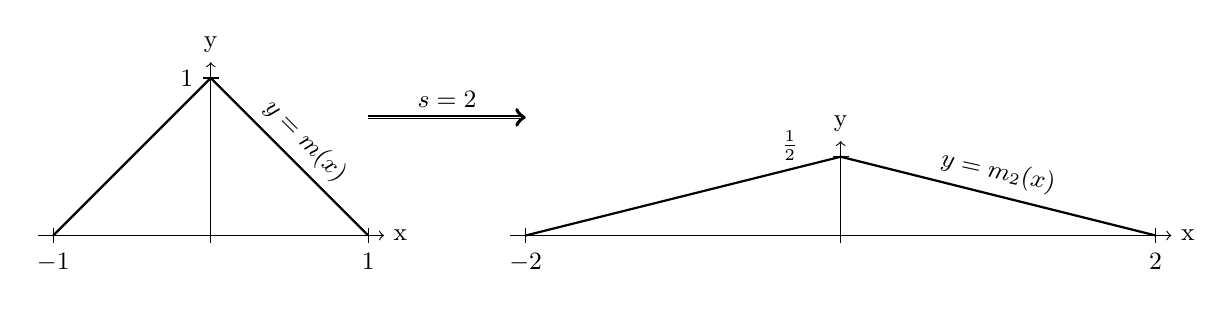
\begin{tikzpicture}
            \draw[->] (-2.2,0) -- (2.2,0) node[right] {\small x};
            \draw[->] (0,-0.1) -- (0,2.2) node[above] {\small y};
            \draw (-2,0.1) -- (-2,-0.1) node[below] {\small $-1$};
            \draw (2,0.1) -- (2,-0.1) node[below] {\small $1$};
            \draw (0.1,2) -- (-0.1,2) node[left] {\small $1$};
            \draw[thick] (-2,0) -- (0,2) -- (2,0);
            \draw (1.2,1.2) node[rotate = -45] {\small $y=m(x)$};
            \draw[->] (3.8,0) -- (12.2,0) node[right] {\small x};
            \draw[->] (8,-0.1) -- (8,1.2) node[above] {\small y};
            \draw (4,0.1) -- (4,-0.1) node[below] {\small $-2$};
            \draw (12,0.1) -- (12,-0.1) node[below] {\small $2$};
            \draw (8.1,1) -- (7.9,1) node[left, xshift = -9, yshift = 4] {\small $\frac{1}{2}$};
            \draw[thick] (4,0) -- (8,1) --(12,0);
            \draw (10,0.8) node[rotate = -12.5] {\small $y=m_2(x)$};
            \draw[->,double] (2,1.5) -- node[above] {\small $s=2$} (4,1.5);
        \end{tikzpicture}
    \end{center}

    Bsp: Gauß-Kern $G(x) = \frac{1}{(2 \pi)^{\frac{d}{2}}} \e^{\frac{-\abs{x}^2}{2}}$\\
    Skalierung mit Faktor $s > 0$
    $$ \Rightarrow G_s(x) = \frac{1}{s^d} G\left( \frac {x} {s} \right) = \frac{1}{s^d} \frac{1}{(2 \pi)^{\frac{d}{2}}} \e^{\frac{-\abs{x}}{2}} = \frac{1}{(2 \pi s^2)^{\frac{d}{2}}} \e^{\frac{-\abs{x}^2}{2s^2}}$$

    Skalierung $s$ $\hat{=}$ Standardabweichung $\sigma$:

    \begin{center}
        \begin{tikzpicture}
            \draw[scale=1,domain=-2.5:2.5,smooth,variable=\x]  plot ({\x},{(e^((-(\x)^2)/2)});
            \draw[scale=1,domain=-2.5:2.5,smooth,variable=\x,shift={(6,0)}]  plot ({\x},{(1/(2*pi)^(1/2))*e^((-(\x)^2)/2)});
            \draw[->,double] (2.5,0.5) -- (3.5,0.5);
        \end{tikzpicture}
    \end{center}

    \subsection{Differenzenfilter}

    Bisher: Glättung $\widehat =$ Mittelwert bilden $\widehat =$ Summe/Integrale\\
    Jetzt: Schärfen $\widehat =$ Differenzen/Kontraste hervorheben $\widehat =$ Differenzen/Ableitungen\\
    \hfill

    \textbf{\large{Diskretisierung von Ableitungen durch Differenzenquotienten:}}

    \hfill
    \begin{minipage}[c]{0.2\linewidth}
        \begin{center}
            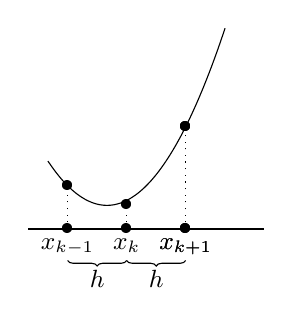
\begin{tikzpicture}
                \draw[scale=1,domain=-0.75:1.5,smooth,variable=\x]  plot ({\x},{(\x * \x)});
                \draw[] (-1,-0.3) -- (2,-0.3);
                \draw[dotted] (-0.5,-0.3) node[] {\small \textbullet} node[below] {\small $x_{k-1}$} -- (-0.5,0.25) node[] {\small \textbullet};
                \draw[dotted] (0.25,-0.3) node[] {\small \textbullet} node[below] {\small $x_{k}$} -- (0.25,0.0125) node[] {\small \textbullet};
                \draw[dotted] (1,-0.3) node[] {\small \textbullet} node[below] {\small $x_{k+1}$} -- (1,1) node[] {\small \textbullet};
                \draw[decorate,decoration={brace,amplitude=2pt,mirror}] (-0.5,-0.7) -- node[below] {\small $h$} (0.25,-0.7);
                \draw[dotted] (1,-0.3) node[] {\small \textbullet} node[below] {\small $x_{k+1}$} -- (1,1) node[] {\small \textbullet};
                \draw[decorate,decoration={brace,amplitude=2pt,mirror}] (0.25,-0.7) -- node[below] {\small $h$} (1,-0.7);
            \end{tikzpicture}
        \end{center}
    \end{minipage}
    \hfill\vrule\hfill
    \begin{minipage}[c]{0.79\linewidth}
        Hier bedeutet $f(k) = f(x_k)$\\
        \begin{align*}
            \text{Vorwärts:}& &u_V^{(1)}(k) & \eqqcolon \frac{f(k+1) - f(k)}{h} & \Rightarrow& &u_V^{(1)} &= \frac{1}{h}\begin{tabular}{|c|c|c|}
                \hline
                0 & -1 & 1\\
                \hline
            \end{tabular} \boxast f\\
            \text{Rückwärts:}& &u_R^{(1)}(k) & \eqqcolon \frac{f(k) - f(k-1)}{h} & \Rightarrow& &u_R^{(1)} &= \frac{1}{h}\begin{tabular}{|c|c|c|}
                \hline
                -1 & 1 & 0\\
                \hline
            \end{tabular} \boxast f\\
            \text{Zentral:}& &u_Z^{(1)}(k) & \eqqcolon \frac{f(k+1) - f(k-1)}{2h} & \Rightarrow& &u_Z^{(1)} &= \frac{1}{2h}\begin{tabular}{|c|c|c|}
                \hline
                -1 & 0 & 1\\
                \hline
                \end{tabular} \boxast f
        \end{align*}
    \end{minipage}

    \hfill

    \textbf{\large{2. Ableitung:}}
    \begin{align*}
        u^{(2)}(k) \approx & \frac{f'(k+1) - f'(k)}{h} \text{(vorwärts)}\\
        \approx & \frac{\frac{f(k+1) - f(k)}{h} - \frac{f(k) - f(k-1)}{h}}{h} \text{(rückwärts)} \\
        = & \frac{f(k+1) -2 f(k) + f(k+1)}{h^2}
    \end{align*}

    Also folgt $\displaystyle u^{(2)} \coloneqq \begin{tabular}{|c|c|c|}
        \hline
        1 & -2 & 1\\
        \hline
        \end{tabular} \boxast f$ und $\displaystyle \frac{1}{h^2}\begin{tabular}{|c|c|c|}
            \hline
            1 & -2 & 1\\
            \hline
            \end{tabular} = \frac{1}{h}\begin{tabular}{|c|c|c|}
                \hline
                0 & -1 & 1\\
                \hline
                \end{tabular} * \frac{1}{h}\begin{tabular}{|c|c|c|}
                    \hline
                    -1 & 1 & 0\\
                    \hline
                    \end{tabular}$\\
    Denn:
    \begin{align*}
        \frac{1}{h} \filter{0 & 1 & -1} * \left(\frac{1}{h} \filter{1 & -1 & 0} * f\right)\\
        =& \left(\frac{1}{h} \filter{ 0 & 1 & -1} * \frac{1}{h} \filter{1 & -1 & 0}\right)*f\\
        =& \left(\frac{1}{h} \filter{ -1 & 1 & 0} \boxast \frac{1}{h} \filter{1 & -1 & 0}\right)*f\\
        =& \frac{1}{h^2} \filter{1 & -2 & 1} * f \\
        =&\frac{1}{h^2} \filter{1 & -2 & 1} \boxast f
    \end{align*}

    In 2D: $\displaystyle \frac{\partial}{\partial x} \widehat = \ \begin{tabular}{|c|c|c|}
        \hline
        0 & -1 & 1\\
        \hline
    \end{tabular}, \ \frac{\partial}{\partial y} \widehat = \begin{tabular}{|c|}
        \hline
        0\\
        \hline
        -1\\
        \hline
        1\\
        \hline
    \end{tabular}, \ \frac{\partial^2}{\partial x^2} \widehat = \begin{tabular}{|c|c|c|}
        \hline
        1 & -2 & 1\\
        \hline
    \end{tabular}, \ \frac{\partial^2}{\partial y^2} \widehat = \begin{tabular}{|c|}
        \hline
        1\\
        \hline
        -2\\
        \hline
        1\\
        \hline
    \end{tabular}$.\\
    \ \\
    \textbf{Diskreter Laplace Operator}\index{Diskreter Laplace Operator}:
    \[\Delta = \frac{\partial^2}{\partial x^2} + \frac{\partial^2}{\partial y^2} \widehat = \ \begin{tabular}{|c|c|c|}
        \hline
        1 & -2 & 1\\
        \hline
    \end{tabular} + \begin{tabular}{|c|}
        \hline
        1\\
        \hline
        -2\\
        \hline
        1\\
        \hline
    \end{tabular} = \begin{tabular}{|c|c|c|}
        \hline
         0 & 1 & 0\\
        \hline
        1 & -4 & 1\\
        \hline
         0 & 1 & 0\\
        \hline
    \end{tabular}\]

    \subsection{Glättungsfilter und partielle Differentialgleichungen}

    Wir haben gesehen: $\displaystyle m = \frac{1}{5}\begin{tabular}{|c|c|c|}
        \hline
        0 & 1 & 0\\
        \hline
        1 & 1 & 1\\
        \hline
        0 & 1 & 0\\
        \hline
    \end{tabular}$ ist unter allen 5-Punkt Filtern der am besten glättende.\\
    Idee: Rauschen weiter verringern indem man $m \boxast$ wiederholt anwendet $\Rightarrow$ Folge von Bildern:\\
    \begin{center}
        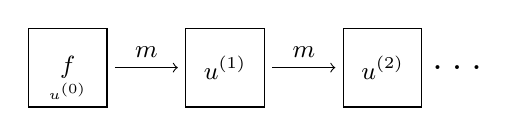
\begin{tikzpicture}
            \draw (0,0) rectangle (1,1);
            \draw (0.5,0.5) node {\small $f$};
            \draw (0.5,0.2) node {\tiny $ \coloneqq  u ^{(0)}$};
            \draw[->] (1.1,0.5) -- node[above] {\small $m \boxast$}(1.9,0.5);
            \draw (2,0) rectangle (3,1);
            \draw (2.5,0.5) node {\small $u^{(1)}$};
            \draw[->] (3.1,0.5) -- node[above] {\small $m \boxast$}(3.9,0.5);
            \draw (4,0) rectangle (5,1);
            \draw (4.5,0.5) node {\small $u^{(2)}$};
            \draw (5,0.5) node[right] {\LARGE \dots};
        \end{tikzpicture}
    \end{center}
    \begin{align*}
        \Rightarrow u^{(n+1)} - u^{(n)} & \hat = \text{\quo{Unterschied zwischen 'Zeit' Punkt $n$ und $n+1$}}\\
        & \hat = \underbrace{m \boxast u^{(n)}}_{u^{n+1}} - \underbrace{\delta \boxast u^{(n)}}_{u^{(n)}} \text{mit } \delta = \begin{tabular}{|c|c|c|}
            \hline
            0 & 0 & 0\\
            \hline
            0 & 1 & 0\\
            \hline
            0 & 0 & 0\\
            \hline
        \end{tabular}\\
        &=(m - \delta) \boxast u^{(n)}\\
        &=\left( \frac{1}{5}\begin{tabular}{|c|c|c|}
            \hline
            0 & 1 & 0\\
            \hline
            1 & 1 & 1\\
            \hline
            0 & 1 & 0\\
            \hline
        \end{tabular} - \frac{1}{5} \begin{tabular}{|c|c|c|}
            \hline
            0 & 0 & 0\\
            \hline
            0 & 5 & 0\\
            \hline
            0 & 0 & 0\\
            \hline
        \end{tabular}\right) \boxast u^{(n)}\\
        &= \frac{1}{5} \begin{tabular}{|c|c|c|}
            \hline
            0 & 1 & 0\\
            \hline
            1 & -4 & 1\\
            \hline
            0 & 1 & 0\\
            \hline
        \end{tabular} \boxast u^{(n)}
    \end{align*} 
    Somit gilt insgesamt:
    \begin{equation}\label{eq:5.11}
        \underbrace{u^{(n+1)} - u^{(n)}}_{\widehat = \frac{\partial u}{\partial t}} = \underbrace{\frac{1}{5} \begin{tabular}{|c|c|c|}
            \hline
            0 & 1 & 0\\
            \hline
            1 & -4 & 1\\
            \hline
            0 & 1 & 0\\
            \hline
        \end{tabular}}_{\widehat = \Delta u}
    \end{equation}

    Kontinuierlich: Funktion $u$
    \[u(x,t) \quad x \in \R^2, \ t \text{ Zeit} \]

    \eqref{eq:5.11} ist eine Diskretisierung (1 Zeitschritt im Eulerverfahren) der partiellen Differentialgleichungen
    \begin{equation}\label{eq:5.12}
        \frac{\partial u}{\partial t} = \Delta u
    \end{equation}
    Bekannt als \textbf{Wärmegleichung}\index{Wärmegleichung} oder \textbf{Diffusionsgleichung}\index{Diffusionsgleichung}.\\
    Zum Zeitpunkt $t=0$ möge die Anfangsbedingung
    \begin{equation}\label{eq:5.13}
        u(x,0)=u^{(0)}=f(x)
    \end{equation}
    gelten. Voranschreiten der Zeit $t$ repräsentiert Diffusion.\\
    Für einen stationären Zustand, also keine Änderung $\frac{\partial u}{\partial t}$ dann muss auch $\Delta u =0$ gelten.\\
    Diese wird unter anderem von konstanten Funktionen oder linearen Funktionen $u(x_1,x_2) = ax_1 + bx_2$ erfüllt.\\
    \ \\
    Es existiert auch einen explizite Formel für die Lösung der Diffusionsgleichung \eqref{eq:5.12} mit Anfangsbedingung \eqref{eq:5.13}:
    \[u(x,t) = \left( G_{\sqrt{2t}} * u^{(0)} \right)(x)\]
    Wobei $\sqrt{2t}$ für eine Skalierung um diesen Wert steht.\\
    Zu zeigen ist: $\displaystyle \frac{\partial u}{\partial t} = \Delta u$
    \[\frac{\partial}{\partial t}  \left( G_{\sqrt{2t}} * u^{(0)} \right) = \Delta  \left( G_{\sqrt{2t}} * u^{(0)} \right)\]
    \[\overset{\text{mit Satz}}{\Longrightarrow}  \left( \frac{\partial}{\partial t} G_{\sqrt{2t}} \right)* u^{(0)} =  \left( \Delta G_{\sqrt{2t}} \right) * u^{(0)}\]
    Es bleibt somit z.z.: $\frac{\partial}{\partial t} G_{\sqrt{2t}} = \Delta G_{\sqrt{2t}}$.

    \begin{center}
        \begin{tikzpicture}
            \draw (0,1.5) node[left] {$t=0$:};
            \draw (0,0) -- (3,0) node[below] {\small a} -- (3,1) -- (4,1) -- (4,0) node[below] {\small b} -- (7,0);
            \draw (0,-2) node[left] {$t>0$:};
            \draw[shift={(0,-3.5)}] plot [smooth, tension = 0.1] coordinates {(0,0) (2.95,0.05) (3.05,1) (3.95,1) (4.05,0.05) (7,0)};
        \end{tikzpicture}
    \end{center}
    Bemerkenswert ist das, für $t=0$ die Funktion nicht stetig ist, aber für alle $t>0$ die Funktion beliebig oft differenzierbar ist.\\
    \ \\
    Insgesamt lässt sich die Idee darstellen als:

    \begin{center}
        \begin{tikzpicture}
            \draw[->] (0,0) node[left] {\small kontinuierlich:} -- (10,0) node[right] {\small t};
            \draw (1,-0.5) rectangle node[] {\large $u^{(0)}$} (2,-1.5);
            \draw (1.5,-1.5) node[below] {\small $u(\cdot,0)$};
            \draw[->] (1.5,-2) -- (1.5,-2.5) -- node[above] {\small $G_{\sqrt{2t}}*$} (8.5,-2.5) -- (8.5,-2);
            \draw (8,-0.5) rectangle  node[] {\large $u^{(t)}$}(9,-1.5);
            \draw (8.5,-1.5) node[below] {\small $u(\cdot,t)$};
            \draw (0,-4) node[left] {\small diskret:};
            \draw (1,-4) rectangle (2,-5);
            \draw (1.5,-4.5) node[] {\large $u^{(0)}$};
            \draw[->] (2.1,-4.5) -- node[above] {\small $m \boxast$} (2.9,-4.5);
            \draw[shift={(2,0)}] (1,-4) rectangle (2,-5);
            \draw[shift={(2,0)}] (1.5,-4.5) node[] {\large $u^{(1)}$};
            \draw[->,shift={(2,0)}] (2.1,-4.5) -- node[above] {\small $m \boxast$} (2.9,-4.5);
            \draw (6,-4.5) node[] {\LARGE \dots};

            \draw[shift={(7,0)}] (1,-4) rectangle (2,-5);
            \draw[shift={(7,0)}] (1.5,-4.5) node[] {\large $u^{(n)}$};
            \draw[->,shift={(5,0)}] (2.1,-4.5) -- node[above] {\small $m \boxast$} (2.9,-4.5);
        \end{tikzpicture}
      \end{center}
      % TODO ???
      \subsection{Isotrope und anisoptrope Diffusion}
      Wir haben gesehen: Glättung/Diffusion verringert Rauschen.\\
      Aber: Auch Kanten/Details werden verwischt.\\
      Ausweg: Diffusion steuern, so dass sie an Kanten (also Stellen mit großer Änderungsrate) weniger stark glättet.\\

      Der Plan lautet also:
      \[\nabla u = \norm{\srmatrix{\frac{\partial u}{\partial x}\\ \frac{\partial u}{\partial y}}}^2 = \begin{cases}
          \text{groß} & \Rightarrow \text{wenig Diffusion}\\
          \text{klein} & \Rightarrow \text{Diffusion normal}
      \end{cases}\]

      Diffusionsgleichung:
      \begin{equation}\label{eq.5.14}
          \frac{\partial u}{\partial t} = \Delta u = \frac{\partial}{\partial x} \frac{\partial}{\partial x} u + \frac{\partial}{\partial y} \frac{\partial}{\partial y} u = \underbrace{\srmatrix{ \frac{\partial }{\partial x } \frac{\partial}{\partial y}}}_{\div{}} \srmatrix{\frac{\partial}{\partial x} u = \frac{\partial}{\partial y} u} = \div(\nabla u)
      \end{equation}

      Um diese Gleichung zu regulieren setzen wir einen \textbf{Diffusionstensor}\index{Diffusionstensor} $M$ in die Gleichung \eqref{eq.5.14} in.
      \[\Delta u = \div(M \nabla u) = \div(\srmatrix{* & * \\ * & *} \nabla u)\]

      Ansätze für $M$:
      \begin{enumerate}[label=\alph*)]
          \item $M=I=\srmatrix{1 & 0 \\ 0 & 1} \Rightarrow$ übliche Diffusion
          \item $M=g_{\kappa}(\norm{\nabla u(x,y)}) \C I$
          \begin{center}
              \begin{tikzpicture}
                  \draw[shift={(-0.75,0.75)}] (0,0) node[left] {$\displaystyle g_\kappa(s) = \frac{1}{1+\left(\frac{s}{\kappa}\right)^2}$};
                  \draw[scale=1.5,domain=0:3,smooth,variable=\x] plot ({\x},{(1/(1+\x*\x)});
                  \draw (0,1.5) node[left] {\small 1};
                  \draw[->] (0,-0.5) -- (0,2);
                  \draw[->] (0,0) -- (5,0) node[right] {\small $s$};
                  \draw[dotted] (1.5,0) node [below] {\small $\kappa$} -- (1.5,0.75);
                  \draw[dotted] (0,0.75) node[left] {\small $\frac{1}{2}$} -- (1.5,0.75);
              \end{tikzpicture}
          \end{center}
          Diese Methode geht zurück auf Perona \& Malik (\textbf{Perona-Malik-Filter}\index{Perona-Malik-Filter} ).
          \begin{enumerate}[label=\textbullet]
              \item Kanten mit $\norm{\nabla u} < \kappa$ werden mehr geglättet
              \item Kanten mit $\norm{\nabla u} \geq \kappa$ werden weniger geglättet
          \end{enumerate}
          Diese Art der Glättung ist \textbf{Isotrop}\index{Isotrop} $\widehat = $ in alle Richtungen gleich starker Fluss.
          \item $M= \begin{pmatrix}
              g\bigl(|\frac{\partial u}{\partial x}(x,y)|\bigr) & 0 \\
              0 & g\bigl(|\frac{\partial u}{\partial y}(x,y)|\bigr)
          \end{pmatrix}$\\
          Diese Art der Diffusionstensoren ist \textbf{anisoptrop}\index{anisoptrop} also richtungsabhängig.\\
          \ \\
          Für $\x \in \Z^2$ und $\x_W = \x + \srmatrix{-1 \\ 0}$ usw.\\
          \begin{center}
              \begin{tikzpicture}
                  \draw (0,0) rectangle node[] {$\x$} (0.5,0.5);
                  \draw[->] (0.25,0.5) -- ++(0,1);
                  \draw (0,1.5) rectangle node[] {$\x_N$} (0.5,2);
                  \draw[->] (0.25,0) -- ++(0,-1);
                  \draw (0,-1) rectangle node[] {$\x_S$} (0.5,-1.5);
                  \draw[->] (0.5,0.25) -- ++(1,0);
                  \draw (1.5,0) rectangle node[] {$\x_O$} (2,0.5);
                  \draw[->] (0,0.25) -- ++(-1,0);
                  \draw (-1,0) rectangle node[] {$\x_W$} (-1.5,0.5);
                  \draw[->] (-1,-0.25) -- ++(0.75,0) node[right] {\small $x$};
                  \draw[->] (-1,-0.25) -- ++(0,-0.75) node[below] {\small $y$};
              \end{tikzpicture}
        \end{center}
        \[\text{Für} \ M=\begin{pmatrix}
            c_1(\x) & 0\\
            0 & c_2(\x)
        \end{pmatrix} \ \text{gilt:}\]

        \begin{align*}\div(M \cdot \nabla u(\x)) =& \begin{pmatrix}
            \frac{\partial}{\partial x} & \frac{\partial}{\partial y}
        \end{pmatrix}
        \left[ \begin{pmatrix}
        c_1(\x) & 0\\
        0 & c_2(\x)
        \end{pmatrix}
        \begin{pmatrix}
            \frac{\partial u}{\partial x} (\x)\\
            \ \\
            \frac{\partial u}{\partial y} (\x)
        \end{pmatrix}
        \right]
        = \begin{pmatrix}
        \frac{\partial}{\partial x} & \frac{\partial}{\partial y}
        \end{pmatrix}
        \begin{pmatrix}
            c_1(\x) \frac{\partial u}{\partial x} (\x)\\
            \ \\
            c_2(\x) \frac{\partial u}{\partial y} (\x)
        \end{pmatrix}\\
        \approx & \begin{pmatrix}
        \frac{\partial}{\partial x} & \frac{\partial}{\partial y}
        \end{pmatrix}
        \begin{pmatrix}
            c_1(\x) (u(\x_O) - u(\x)) \\
            \ \\
            c_2(\x) (u(\x_S) - u(\x))
        \end{pmatrix}\\
        \approx & c_1(\x) (u(\x_O) - u(\x)) - c_1(\x_W)(u(\x_N) - u(\x_W))\\
        +&c_2(\x) (u(\x_S) - u(\x)) - c_2(\x_N)(u(\x) - u(\x_N))
        \end{align*}
      \end{enumerate}

      \subsection{Bilaterale Filter}
      Es existiert auch ein anderer Ansatz für das selbe Problem.
      \[u(\x) = \text{ gewichtetes Mittel aus allen } f(\y) \text{ mit}\]

      \begin{enumerate}[label= \alph*)]
          \item $\y$ ist nahe bei $\x$ \underline{und}
          \item $f(\y)$ ist nahe bei $f(\x)$
      \end{enumerate}

      \[u(\x) = \frac{1}{w(\x)} \int_\Omega \underbrace{g(\x - \y)}_{a)} \underbrace{h(f(\x) - f(\y))}_{\text{neu }b)} f(\y) d\y\]
      Heißt \textbf{Bilateraler Filter}\index{Bilateraler Filter}, wobei
      \[w(\x) = \int_\Omega g(\x - \y) h(f(\x) - f(\y)) d\y\]

      \begin{enumerate}
          \item[Oft:] $g,h$ Gauß-Kerne ($\Rightarrow$ nichtlineare Gaußfilter)
          \item[Manchmal:] $g,h$ charakteristische Funktionen ($\Rightarrow$ SUSAN-Filter)
          \begin{enumerate}
              \item[Effekt:] Falls Höhe der Kante $>$ Filterradius $\Rightarrow$ Kante bleibt
          \end{enumerate}
          \item[Manchmal:] $f \overset{\log}{\mapsto} \log \ f \overset{\small \text{Bil. Filter}}{\mapsto} \log \ u \overset{exp}{\mapsto} u$
      \end{enumerate}
      Diese Verfahren ist jedoch sehr aufwendig, denn
      \begin{enumerate}[label=\textbullet]
          \item keine reine Filterung ($\Rightarrow$ keine FFT-Implementierung möglich)
          \item Normalisierung $w(\x)$ in jedem Punkt berechnen
      \end{enumerate}

      \subsection{Entrauschen mittels Variationsrechnung}
      Erinnerung:
      \begin{center}
          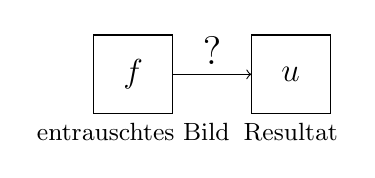
\begin{tikzpicture}
              \draw (0,0) rectangle node[] {\large $f$} (1,1);
              \draw (0.5,0) node[below] {\small entrauschtes Bild};
              \draw[->] (1,0.5) -- node[above] {\Large ?} (2,0.5);
              \draw (2,0) rectangle node[] {\large $u$} (3,1);
              \draw (2.5,0) node[below] {\small Resultat};
          \end{tikzpicture}
      \end{center}

      Wünsche an $u$:
      \begin{enumerate}
          \item $u \approx f$ (Datenkonsistenz)
          \item $u$ ist 'glatt'. (Regularitätsbedingung)
      \end{enumerate}

      Mathematische Umsetzung der Wünsche:
      \begin{enumerate}
          \item $\displaystyle \norm{u-f}_2 = \sqrt{\int_\Omega \abs{u(\x) - f(\x)}^2 \d x}$ sei klein
          \item $\displaystyle \norm{\nabla u}_2 = \sqrt{\int_\Omega \abs{\nabla u(\x)}^2 \d x} = \sqrt{\int_\Omega \left( \frac{\partial u}{\partial x} (\x) \right)^2 + \left( \frac{\partial u}{\partial y} (\x) \right)^2 d\x} $ sei klein
      \end{enumerate}

      Kombination:
      \begin{equation}\label{eq:5.15}
          J(u)  \coloneqq  \norm{u-f}_2^2 + \lambda \norm{\nabla u}_2^2 \overset{u \in U}{\rightarrow} \text{min}
      \end{equation}
      Für einen geeigneten Funktionen Raum $U$ und \textbf{Kopplungskonstante}\index{Kopplungskonstante} $\lambda > 0$.\\
      In diesem Beispiel empfiehlt sich als Suchraum:
      \[U=\{ u : \norm{u}_2 < \infty, \ \nabla u \text{ existiert }, \ \norm{\nabla u}_2<\infty  \}=W^{1,2}\]
      ein so genannter \textbf{Sobolev-Räume}\index{Sobolev-Räume}. Diese Suchproblem is jedoch $\infty$-dimensional und somit schwer zu lösen.\\
      Im obigen Ansatz \eqref{eq:5.15} stellt man fest, dass der Regularitätsterm
      \[\norm{\nabla u}_2^2 = \int_\Omega \abs{\nabla u(\x)}^2 d\x =
      \int_\Omega \left( \frac{\partial u}{\partial x} (\x) \right)^2 + \left( \frac{\partial u}{\partial y} (\x) \right)^2 d\x \]
      die großen Gradienten an (gewollten) Kanten zu stark bestraft. ($\Rightarrow$ optimales $u$ glättet Kanten)\\

      Ausweg: Wähle $\norm{\nabla u}_2$ oder $\displaystyle \norm{\nabla u}_1 =\int_\Omega \abs{\nabla u(\x)} d\x = \int_\Omega \abs{\frac{\partial u}{\partial x} (\x)} + \abs{\frac{\partial u}{\partial y} (\x)} d\x$ als Regularitätsterme.

      \begin{equation}\label{eq:5.16}
        J(u) \coloneqq  \norm{u-f}_2^2 + \lambda \norm{\nabla u}_1 \to \ \text{min}
      \end{equation}
      Genannt \textbf{Rudin–Osher–Fatemi-Funktional}\index{Rudin–Osher–Fatemi-Funktional} (ROF)

      \textbf{Allgemeiner Ansatz bei Variationsproblemen:}

      \[J(u) \coloneqq \underbrace{D(u,f)}_{\text{Datenkern}} + \lambda \underbrace{R(u)}_{\text{Regularitätsterm}} \overset{u \in U}{\to} \text{min}\]

      Notwendiges Kriterium:\\
      Falls $J:U \to \R$ in $u \in U$ ein lokales Minimum besitzt, dann gilt für jede Richtung $v \in U$:
      \begin{equation}\label{eq:5.17}
        \underset{\epsilon \nearrow 0}{\lim} \frac{J(u+\epsilon v) - J(u)}{\epsilon}=0
      \end{equation}
      Dies ist die Verallgemeinerte Richtungsableitung (Gateux-Ableitung).\\

      Häufig ist $J$ in Integralform gegeben, z.b.:
      \[J(u)= \int_\Omega g(x,u(x),\nabla(x)) \d x.\]
      Dann führt Bedingung \eqref{eq:5.17} auf Gleichungen für bestimmte partielle Ableitungen von $g$ und $u$, die sogenannte \textbf{Euler-Lagrange-Gleichung}\index{Euler-Lagrange-Gleichung} für \eqref{eq:5.17}.\\
      $\Rightarrow$ partielle Differentialgleichung für $u$.

      Fazit:
      \begin{center}
          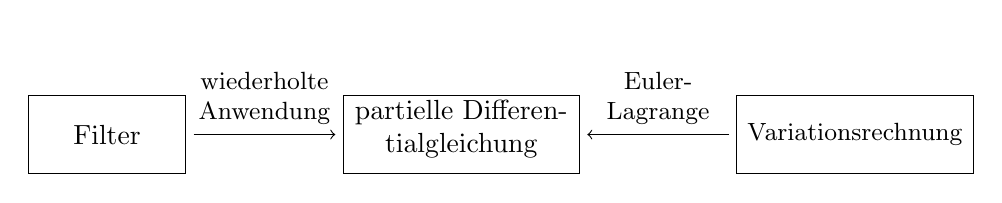
\begin{tikzpicture}
              \draw (0,0) rectangle node[] {Filter} (2,1);
              \draw[->] (2.1,0.5) -- node[above, text width=2cm] {\small \begin{center}
                wiederholte Anwendung
              \end{center}} (3.9,0.5);
              \draw (4,0) rectangle node[yshift=-12,above,text width=3cm] {\begin{center}
                partielle Differentialgleichung
              \end{center}} (7,1);
              \draw[->] (8.9,0.5) -- node[above,text width=2cm] {\small \begin{center}
                Euler-Lagrange
              \end{center}} (7.1,0.5);
              \draw (9,0) rectangle node[] {\small Variationsrechnung} (12,1);
          \end{tikzpicture}
      \end{center}
